% !TEX root = ../preview.tex

\section{Method}
\label{sec:method}

% This file mirrors 3_Method.md. Keep both versions aligned.

\subsection{Feedback Flow Matching with Overlapping Chunks}
\label{sec:method:overlap}

FBFM turns chunked WAM inference into a feedback process without modifying or
retraining the pretrained model. Suppose that a new chunk is generated at
environment time $t$ while its preceding action chunk is still being executed.
After both chunks are aligned to global environment time, let
\begin{equation}
    \mathcal I_t^A
    =
    \left\{
        i\in\{0,\ldots,H-1\}:
        a_{t+i}\text{ is covered by both chunks}
    \right\}
    \label{eq:action-overlap-set}
\end{equation}
denote their overlap. For every $i\in\mathcal I_t^A$, the action inherited from
the preceding chunk is denoted by $a_{t+i}^{\mathrm{prev}}$. It is a committed
action target for the corresponding slot of the new chunk. The committed set
includes both actions that have already been sent to the environment and actions
that remain scheduled for execution from the preceding chunk. Because the robot
continues to execute that chunk in order, the position reached by the execution
pointer does not alter the overlap constraint: the two chunks must agree over the
entire aligned overlap.

Execution and generation proceed concurrently at the level of the method. Executing
$a_{t+i-1}^{\mathrm{prev}}$ produces a real transition whose observation is encoded
as $z_{t+i}$. At the $k$-th solver evaluation, we collect all state feedback that
has arrived by then in
\begin{equation}
    \mathcal F_{t,k}
    =
    \left\{
        (i,z_{t+i}):i\in\{1,\ldots,H\},
        z_{t+i}\text{ is available before solver evaluation }k
    \right\}.
    \label{eq:dynamic-feedback-set}
\end{equation}

The interaction history $\mathcal H_t$ remains the condition available when the
solver is launched. In particular, newly arriving $z_{t+i}$ is not absorbed into
or hidden by a redefinition of $\mathcal H_t$; it is exposed explicitly through the
dynamic feedback set $\mathcal F_{t,k}$ and its corresponding mask. This separation
is central to FBFM: the pretrained conditional model remains fixed, while real
transitions progressively constrain the chunk that is still being generated.

\begin{figure*}[t]
    \centering
    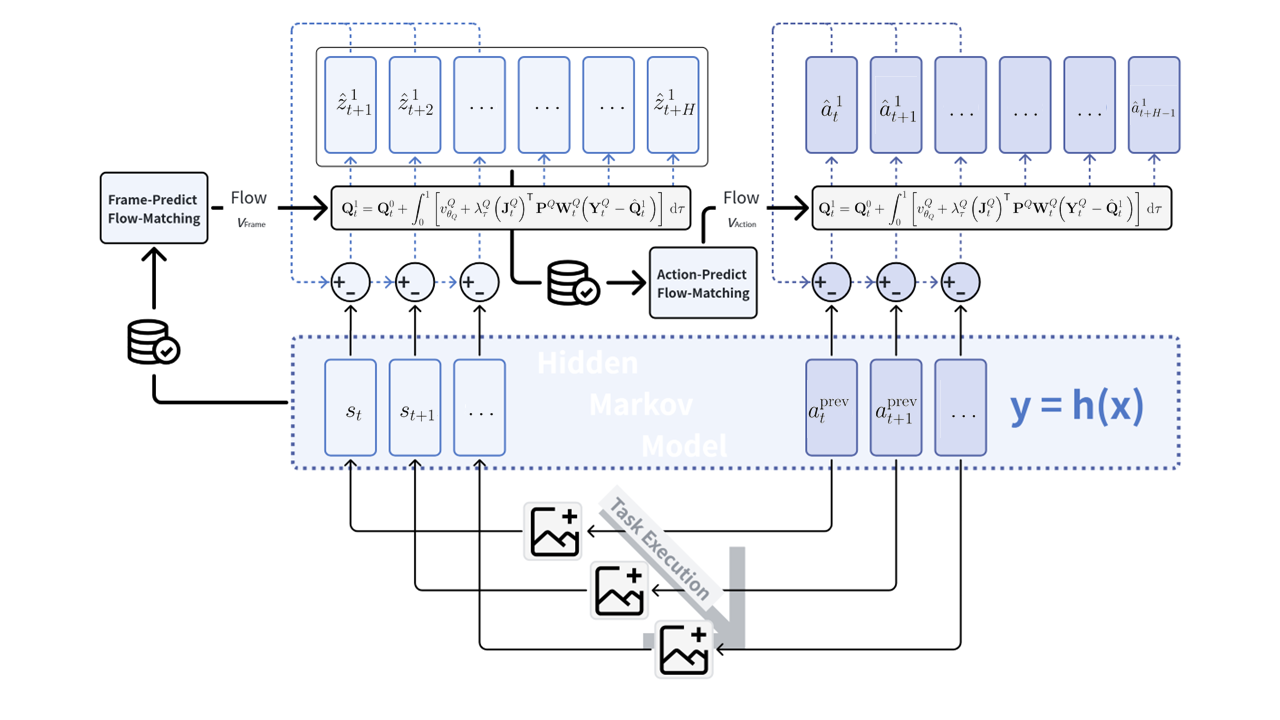
\includegraphics[width=\textwidth]{../material/serial.png}
    \caption{FBFM for a stage-wise WAM. While the preceding chunk is executed,
    encoded real observations progressively constrain the state flow. The latest
    corrected state context conditions the action flow, whose overlap is constrained
    by the committed actions inherited from the preceding chunk.}
    \label{fig:fbfm-stage-wise}
\end{figure*}

\subsection{Unified Pseudoinverse-Guided Flow Correction}
\label{sec:method:unified-guidance}

FBFM adapts pseudoinverse guidance~\cite{song2023pseudoinverse} to the active
flow of a WAM. Let $Q\in\{Z,A,X\}$ indicate whether the generated variable
$\mathbf Q_t\in\mathbb R^{D_Q}$ is a latent-state chunk, an action chunk, or
their joint representation. The corresponding frozen vector field, parameters,
flow time, and native conditioning context are denoted by
$v_{\theta_Q}^Q$, $\theta_Q$, $\tau_k^Q$, and
$\mathcal K_{t,k}^Q$, respectively.

Following the inverse-problem view, a clean variable produces a feedback
measurement
\begin{equation}
    \mathbf m_{t,k}^Q
    =h_Q(\mathbf Q_t^1)+\boldsymbol\eta,
    \qquad
    \boldsymbol\eta\sim\mathcal N(\mathbf 0,\sigma_y^2\mathbf I),
    \label{eq:fbfm-measurement}
\end{equation}
where $h_Q$ maps the generation space to the feedback space and
$h_Q^\dagger$ is its generalized inverse. We interpret them as a
Moore--Penrose-compatible encoder--decoder pair and store the lifted target as
$\mathbf Y_{t,k}^Q:=h_Q^\dagger(\mathbf m_{t,k}^Q)$. Pseudoinverse guidance
compares this target with
$h_Q^\dagger(h_Q(\hat{\mathbf Q}_{t,k}^1))$. Because FBFM feedback and model
predictions are already represented in aligned latent or action coordinates, we
use
$h_Q^\dagger(h_Q(\hat{\mathbf Q}_{t,k}^1))\approx
\hat{\mathbf Q}_{t,k}^1$ on the selected subspace. Appendix~\ref{app:pseudoinverse}
states the corresponding consistency assumptions.

Let $\mathbf W_{t,k}^Q$ select or confidence-weight the constrained
coordinates, and let the separate operator $\mathbf P^Q$ balance their scale.
At every solver evaluation, all FBFM instantiations use the same correction
chain:
\begin{align}
    \hat{\mathbf Q}_{t,k}^1
    &=f_{\theta_Q}^{Q,\tau_k^Q}(\mathbf Q_t^{\tau_k^Q})
    :=\mathbf Q_t^{\tau_k^Q}
    +(1-\tau_k^Q)v_{\theta_Q}^Q
      (\mathbf Q_t^{\tau_k^Q},\tau_k^Q;\mathcal K_{t,k}^Q),
    \label{eq:fbfm-clean-endpoint}\\
    \mathbf e_{t,k}^Q
    &=\mathbf P^Q\mathbf W_{t,k}^Q
      (\mathbf Y_{t,k}^Q-\hat{\mathbf Q}_{t,k}^1),
    \label{eq:fbfm-aligned-error}\\
    \mathbf J_{t,k}^Q
    &:=\frac{\partial\hat{\mathbf Q}_{t,k}^1}
             {\partial\mathbf Q_t^{\tau_k^Q}},
    \qquad
    \mathbf g_{t,k}^Q=(\mathbf J_{t,k}^Q)^{\mathsf T}\mathbf e_{t,k}^Q,
    \qquad
    v_{\mathrm{FBFM}}^Q
    =v_{\theta_Q}^Q+\lambda_{\tau_k^Q}^Q\mathbf g_{t,k}^Q.
    \label{eq:fbfm-guided-field}
\end{align}
Here, $\lambda_{\tau_k^Q}^Q$ is the flow-time-dependent guidance strength.
This formulation follows the Flow-Matching inpainting construction of
Black et al.~\cite{black2025realtime}, while making the support mask and
modality preconditioner explicit. The remainder of this section only specifies
the assignments of
$(\mathbf Q,\theta_Q,\mathcal K,\mathbf Y,\mathbf W,\mathbf P)$ for stage-wise
and joint-generation WAMs.

\subsection{FBFM for Stage-Wise World--Action Models}
\label{sec:method:stage-wise}

A stage-wise WAM factorizes latent-state and action generation as
\begin{equation}
    p_\theta(\mathbf Z_t,\mathbf A_t\mid\mathcal H_t)
    =
    p_{\theta_Z}(\mathbf Z_t\mid\mathcal H_t)
    p_{\theta_A}(\mathbf A_t\mid\mathbf Z_t,\mathcal H_t),
    \label{eq:stage-wise-factorization}
\end{equation}
and realizes the two factors with separate vector fields $v_{\theta_Z}^Z$ and
$v_{\theta_A}^A$. FBFM therefore applies separate state and action corrections,
while passing the corrected state representation to the action stage.

The stage-wise procedure follows the same state-first, action-second order as the
underlying WAM. While the preceding action chunk is being executed, generation of
the new chunk proceeds in two stages. First, as the robot executes the remaining
actions of the preceding chunk within the overlap, each action
$a_{t+i-1}^{\mathrm{prev}}$ induces a transition in the physical or simulated
environment according to $P(\cdot\mid s_{t+i-1},a_{t+i-1}^{\mathrm{prev}})$. The
resulting state is sensed and encoded as $z_{t+i}$, which activates the
corresponding state mask and constrains the ongoing state flow. Second, the action
flow is conditioned on the latest corrected state context and is directly
constrained by the committed actions in the cross-chunk overlap. State feedback
that arrives after the state flow has terminated refreshes the context used by the
ongoing action flow rather than restarting state generation.

Figure~\ref{fig:stage-wise-masked-guidance} makes the resulting separation
explicit: the two stages use distinct endpoint Jacobians and distinct masks, even
though feedback collected during execution connects them temporally.

\begin{figure*}[t]
    \centering
    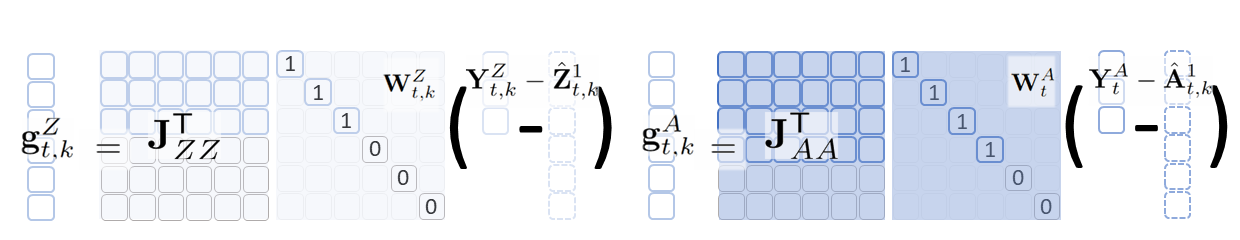
\includegraphics[width=0.98\textwidth]{../material/mask/serial_0_cropped.png}
    \vspace{0.3em}

    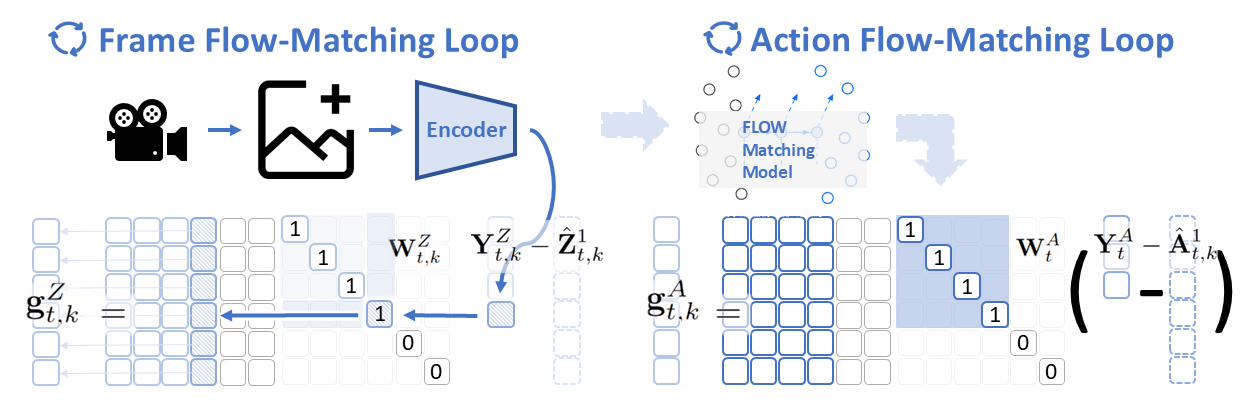
\includegraphics[width=0.98\textwidth]{../material/mask/serial_1_cropped.png}
    \caption{Masked FBFM guidance for a stage-wise WAM: \emph{top,} the state and
    action endpoints are predicted by separate flows, so each discrepancy is
    propagated through its corresponding within-modality endpoint Jacobian;
    \emph{bottom,} real observations progressively activate state-mask entries
    during the latent-state (frame) flow, whereas the subsequent action flow uses
    the fixed mask induced by the aligned cross-chunk action overlap.}
    \label{fig:stage-wise-masked-guidance}
\end{figure*}

\subsubsection{State Flow: Dynamic State-Feedback Guidance}

For the state stage, the unified correction uses
$Q=Z$, $\theta_Q=\theta_Z$,
$\mathcal K_{t,k}^Z=\mathcal H_t$, and
$\mathbf P^Z=P_Z\mathbf I_{D_Z}$. At state-solver flow time
$\tau_k^Z$, we encode $\mathcal F_{t,k}$ as an aligned state-feedback target
$\mathbf Y_{t,k}^Z\in\mathbb R^{D_Z}$ and a block-diagonal mask
\begin{equation}
    \mathbf W_{t,k}^Z
    =
    \operatorname{Diag}
    \!\left(w_{t,1}^{Z,k},\ldots,w_{t,H}^{Z,k}\right)
    \otimes\mathbf I_{d_z}
    \in\mathbb R^{D_Z\times D_Z},
    \qquad
    w_{t,i}^{Z,k}>0
    \Longleftrightarrow
    (i,z_{t+i})\in\mathcal F_{t,k}.
    \label{eq:dynamic-state-mask}
\end{equation}
For an observed slot, the corresponding block of $\mathbf Y_{t,k}^Z$ is
$z_{t+i}$; unobserved blocks may be filled arbitrarily because their weights are
zero. Binary weights impose hard state inpainting, while weights in $[0,1]$
permit confidence-weighted feedback. These assignments are substituted directly
into Eqs.~\eqref{eq:fbfm-clean-endpoint}--\eqref{eq:fbfm-guided-field}; no
separate state-specific guidance rule is required.

Before every state-solver evaluation, $\mathcal F_{t,k}$,
$\mathbf Y_{t,k}^Z$, and $\mathbf W_{t,k}^Z$ are refreshed. Consequently, a
latent state that becomes available during generation affects the remaining solver
steps of the same active chunk rather than waiting for the next inference call.

\subsubsection{Action Flow: State-Context Refresh and Previous-Action Consistency}

\paragraph{State-context refresh.}

After the state flow terminates, let $\hat{\mathbf Z}_t$ be its generated endpoint.
Additional state feedback may arrive while the action flow is still running. At an
action-solver evaluation $k$, we reuse $\mathbf Y_{t,k}^Z$ and
$\mathbf W_{t,k}^Z$ for the latest feedback snapshot available at that evaluation
and form the corrected state representation by
\begin{equation}
    \check{\mathbf Z}_{t,k}
    =
    \left(\mathbf I_{D_Z}-\mathbf W_{t,k}^Z\right)
    \hat{\mathbf Z}_t
    +
    \mathbf W_{t,k}^Z
    \mathbf Y_{t,k}^Z,
    \label{eq:refreshed-state-representation}
\end{equation}
and expose it to the action generator through an abstract state context
\begin{equation}
    \mathcal C_{t,k}^Z
    =
    \Phi_Z(\check{\mathbf Z}_{t,k},\mathcal H_t).
    \label{eq:state-context-interface}
\end{equation}
Here, $\Phi_Z$ denotes the native context-construction interface of the stage-wise
WAM. It may be realized by latent tokens, intermediate features, or an updated
attention memory; FBFM does not require a particular storage mechanism. This
context-refresh condition only specifies how a stage-wise generator consumes late
state feedback. It is not an additional guidance objective or a model-specific part
of FBFM.

\paragraph{Previous-action consistency.}

Let $\mathbf Y_t^A\in\mathbb R^{D_A}$ contain the actions
$a_{t+i}^{\mathrm{prev}}$ aligned to the new action horizon, with arbitrary values
outside $\mathcal I_t^A$. We represent the general previous-action constraint by a
nonnegative weighting operator
\begin{equation}
    \mathbf W_t^A\in[0,1]^{D_A\times D_A},
    \qquad D_A=H d_a,
    \label{eq:general-action-weight}
\end{equation}
whose support lies on the aligned overlap. A common hard-overlap specialization is
\begin{equation}
    \mathbf W_t^A
    =
    \operatorname{Diag}
    \!\left(
        \mathbb 1[0\in\mathcal I_t^A],\ldots,
        \mathbb 1[H-1\in\mathcal I_t^A]
    \right)
    \otimes\mathbf I_{d_a}.
    \label{eq:hard-overlap-action-mask}
\end{equation}

Crucially, $\mathbf Y_t^A$ and $\mathbf W_t^A$ describe cross-chunk consistency,
not the current execution pointer. They therefore remain fixed throughout generation
of the new chunk, regardless of which committed overlap actions have already been
executed.

For the action stage, the unified correction uses
$Q=A$, $\theta_Q=\theta_A$,
$\mathcal K_{t,k}^A=(\mathcal H_t,\mathcal C_{t,k}^Z)$, and
$\mathbf P^A=P_A\mathbf I_{D_A}$, with the fixed assignments
$\mathbf Y_{t,k}^A=\mathbf Y_t^A$ and
$\mathbf W_{t,k}^A=\mathbf W_t^A$. Substituting them into
Eqs.~\eqref{eq:fbfm-clean-endpoint}--\eqref{eq:fbfm-guided-field} makes the
latest refreshed state context condition the endpoint predictor while the overlap
target directly constrains the action flow; no separate action-specific guidance
rule is required.

State feedback and previous-action consistency thus have distinct roles in a
stage-wise WAM. State feedback is asynchronous and progressively updates both the
state flow and the context consumed by the action flow. The previous-action target
is fixed by the temporal overlap and directly constrains the action flow. Their
combination closes the loop within chunk generation while preserving the original
state-first, action-second factorization.

\subsection{FBFM for Joint-Generation World--Action Models}
\label{sec:method:joint}

A joint-generation WAM, also referred to here as a parallel WAM, models the latent
state and action chunks with a single conditional distribution,
\begin{equation}
    p_\theta(\mathbf X_t\mid\mathcal H_t),
    \qquad
    \mathbf X_t
    =
    \begin{bmatrix}
        \mathbf Z_t\\
        \mathbf A_t
    \end{bmatrix}.
    \label{eq:joint-generation-model}
\end{equation}
Unlike a stage-wise WAM, it transports both modalities with one vector field
$v_\theta^X$ and does not require a separate state-to-action context handoff. The
dynamic state feedback and the fixed previous-action target are instead assembled
into one joint constraint and applied at every evaluation of the same Flow-Matching
solver.

\begin{figure*}[t]
    \centering
    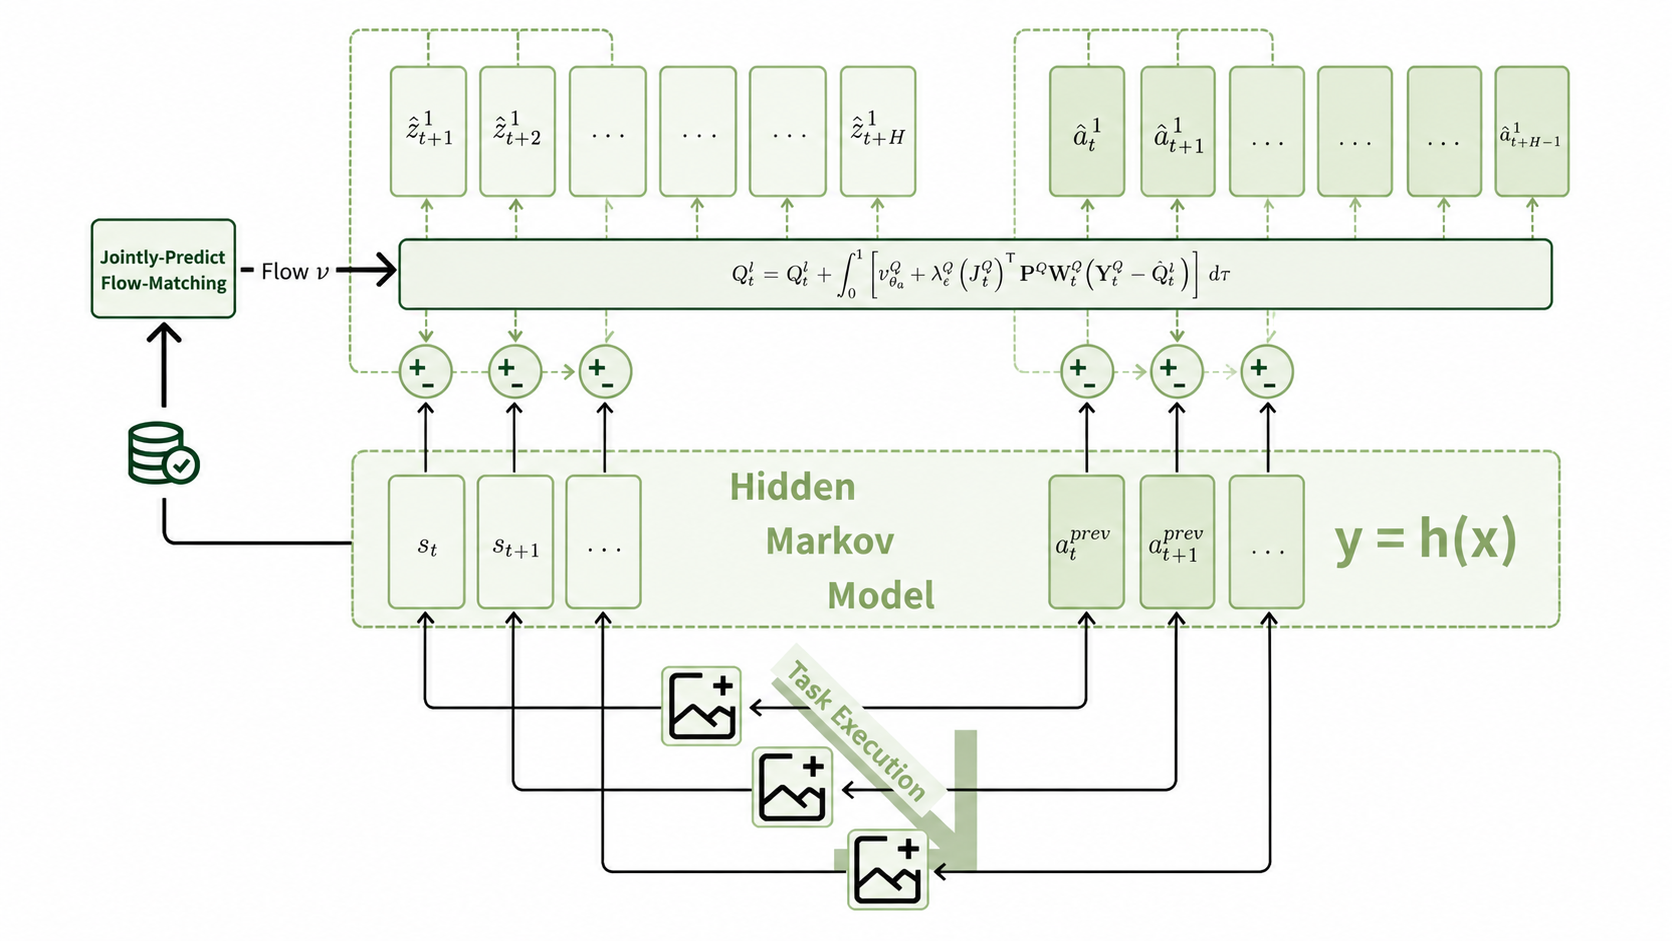
\includegraphics[width=\textwidth]{../material/parallel.png}
    \caption{FBFM for a joint-generation WAM. Encoded transitions observed while
    the preceding chunk is executed and committed actions from the cross-chunk
    overlap jointly constrain a single state-action flow. Through the cross-modal
    blocks of the endpoint Jacobian, state feedback can directly correct the action
    coordinates of this flow.}
    \label{fig:fbfm-joint}
\end{figure*}

\subsubsection{Joint State--Action Guidance}

Using the state-feedback quantities from Section~\ref{sec:method:stage-wise} and
the same aligned previous-action target, we define
\begin{equation}
    \mathbf Y_{t,k}^X
    =
    \begin{bmatrix}
        \mathbf Y_{t,k}^Z\\
        \mathbf Y_t^A
    \end{bmatrix},
    \label{eq:joint-feedback-target}
\end{equation}
and
\begin{equation}
    \mathbf W_{t,k}^X
    =
    \begin{bmatrix}
        \mathbf W_{t,k}^Z & \mathbf 0\\
        \mathbf 0 & \mathbf W_t^A
    \end{bmatrix}
    \in\mathbb R^{D_X\times D_X},
    \qquad
    D_X=D_Z+D_A,
    \quad
    D_Z=H d_z.
    \label{eq:joint-feedback-mask}
\end{equation}

The corresponding modality preconditioner is
\begin{equation}
    \mathbf P^X
    =
    \operatorname{blkdiag}
    \!\left(P_Z\mathbf I_{D_Z},P_A\mathbf I_{D_A}\right).
    \label{eq:joint-preconditioner}
\end{equation}

The state block of $\mathbf W_{t,k}^X$ is refreshed whenever a new
$z_{t+i}$ becomes available, whereas its action block remains fixed by the aligned
cross-chunk overlap. For joint generation, the remaining unified assignments are
$Q=X$, $\theta_Q=\theta$, and $\mathcal K_{t,k}^X=\mathcal H_t$.
Substituting these quantities into
Eqs.~\eqref{eq:fbfm-clean-endpoint}--\eqref{eq:fbfm-guided-field} gives the
complete joint update; no separate joint-specific guidance rule is required.
Thus, one guidance evaluation simultaneously enforces the observed state slots and
the committed action overlap while leaving all unobserved and unconstrained
coordinates to the pretrained joint model.

Figure~\ref{fig:joint-masked-guidance} illustrates both parts of this joint
update: the mask forms modality-specific discrepancies, while the transpose of the
full endpoint Jacobian propagates them across state and action coordinates.

\begin{figure*}[t]
    \centering
    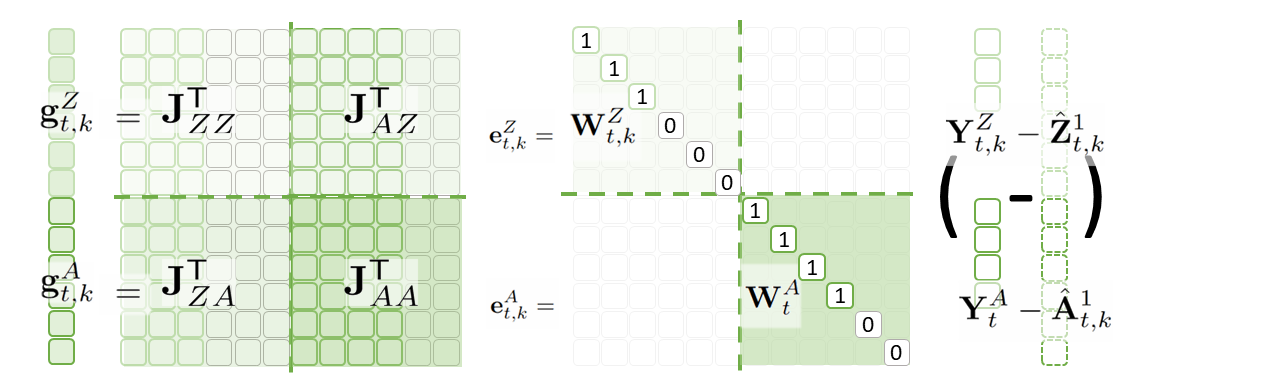
\includegraphics[width=0.98\textwidth]{../material/mask/parallel_0_cropped.png}
    \vspace{0.4em}

    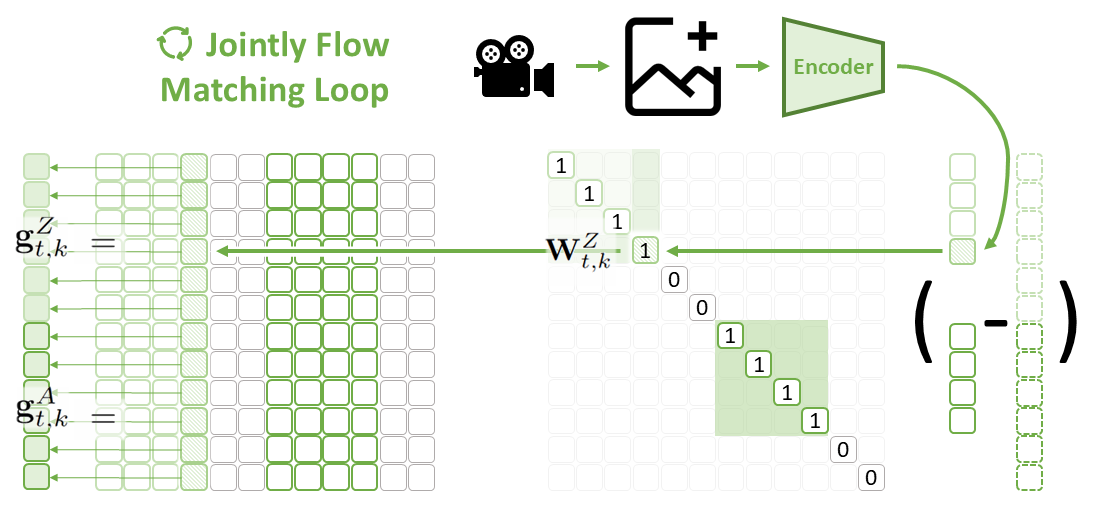
\includegraphics[width=0.98\textwidth]{../material/mask/parallel_1_cropped.png}
    \caption{Masked FBFM guidance for a joint-generation WAM: \emph{top,} the
    block-diagonal feedback mask forms separate state and action discrepancies,
    but the full endpoint-Jacobian transpose maps both into the corrections of
    both modalities; \emph{bottom,} each newly encoded observation activates its
    aligned state-mask entry during the ongoing joint Flow-Matching loop; through
    the cross-modal Jacobian blocks, the resulting correction can directly affect
    the action coordinates. The action-overlap mask remains fixed.}
    \label{fig:joint-masked-guidance}
\end{figure*}

\subsubsection{Direct State-to-Action Correction}

The direct coupling becomes explicit by partitioning the clean-endpoint Jacobian
$\mathbf J_{t,k}^X$ defined in Eq.~\eqref{eq:fbfm-guided-field}:
\begin{equation}
    \mathbf J_{t,k}^X
    =
    \begin{bmatrix}
        \mathbf J_{ZZ} & \mathbf J_{ZA}\\
        \mathbf J_{AZ} & \mathbf J_{AA}
    \end{bmatrix}.
    \label{eq:joint-jacobian-blocks}
\end{equation}
For $Q,R\in\{Z,A\}$, each block is
\begin{equation}
    \mathbf J_{QR}
    =
    \frac{\partial\hat{\mathbf Q}_{t,k}^1}
         {\partial\mathbf R_t^{\tau_k^X}}.
    \label{eq:cross-modal-jacobian-block}
\end{equation}

Partitioning
$\mathbf e_{t,k}^X=[\mathbf e_{t,k}^Z;\mathbf e_{t,k}^A]$ and
$\mathbf g_{t,k}^X=[\mathbf g_{t,k}^Z;\mathbf g_{t,k}^A]$, the VJP gives
\begin{equation}
    \begin{bmatrix}
        \mathbf g_{t,k}^Z\\
        \mathbf g_{t,k}^A
    \end{bmatrix}
    =
    \begin{bmatrix}
        \mathbf J_{ZZ}^{\mathsf T} & \mathbf J_{AZ}^{\mathsf T}\\
        \mathbf J_{ZA}^{\mathsf T} & \mathbf J_{AA}^{\mathsf T}
    \end{bmatrix}
    \begin{bmatrix}
        \mathbf e_{t,k}^Z\\
        \mathbf e_{t,k}^A
    \end{bmatrix}.
    \label{eq:joint-vjp-blocks}
\end{equation}

In particular, consider state feedback alone, for which
$\mathbf e_{t,k}^A=\mathbf 0$. The action component of the correction becomes
\begin{equation}
    \mathbf g_{t,k}^A
    =
    \mathbf J_{ZA}^{\mathsf T}\mathbf e_{t,k}^Z
    =
    \left(
        \frac{\partial\hat{\mathbf Z}_{t,k}^1}
             {\partial\mathbf A_t^{\tau_k^X}}
    \right)^{\mathsf T}
    \mathbf e_{t,k}^Z.
    \label{eq:direct-state-to-action-correction}
\end{equation}

Whenever the learned joint endpoint predictor couples states and actions,
$\mathbf J_{ZA}\neq\mathbf 0$, and a discrepancy in an observed state slot
therefore produces a nonzero correction on the action coordinates in the same
solver step. This is the principal distinction from the stage-wise formulation:
state feedback does not influence action generation only through a subsequently
refreshed context; it can directly modify the action flow through the cross-modal
Jacobian of the joint predictor. The reciprocal cross block also allows an action
residual to affect state coordinates, although FBFM primarily uses the former path
to inject real state transitions into action generation.


\subsection{Training-Free Inference}
\label{sec:method:training-free}

FBFM changes only the inference-time vector fields and context supplied to the
pretrained WAM. The joint parameter set $\theta$, or the stage-wise parameter sets
$\theta_Z$ and $\theta_A$, remain frozen, and the VJPs are obtained by automatic
differentiation through the clean-endpoint predictors.
The method does not require a fixed ratio between environment steps and solver
steps. It only requires feedback available before a solver evaluation to be visible
to that evaluation. The concrete scheduling mechanism is therefore an experimental
property rather than part of the method definition.
